\documentclass[matan]{subfiles}

\begin{document}
  \section{Интегральные суммы Римана. Интегрируемость по Риману.}
  \hypertarget{q1}{}

  \begin{definition}
      $\uptau$-разбиение на $[a;b]$: $$\uptau=\{x_k\}^n_{k=0}: a=x_0<x_1<...<x_n=b$$
  \end{definition}

  \begin{definition}
      Мелкость разбиения $\uptau$: $$\uplambda(\uptau)=\underset{k=0...n-1}{max\ \Delta_k} = x_{k+1}-x_k$$
  \end{definition}

  \begin{definition}
      Оснащение разбиения $\uptau$: $$\xi=\{\xi_k\}^{n-1}_{k=0}: \xi_k \in [x_k, x_{k+1}]$$
  \end{definition}

  \begin{definition}
       Пусть $f: [a, b] \rightarrow \R$, тогда cумма Римана: $$S(f, \uptau, \xi)=\sum\limits_{k=0}^{n-1} f(\xi_k) \Delta_k$$
  \end{definition}

  \begin{definition}
      Интегралом Римана функции $f$ по отрезку $[a, b]$ называется $I \in \R$: $$\forall \E > 0\ \e \updelta > 0: \forall \uptau: \ \uplambda(\uptau) < \updelta,\ \forall \xi \ |S(f, \uptau, \xi) - I| < \E$$ то есть неформально $$\lim_{\uplambda(\uptau) \rightarrow 0} S(f, \uptau, \xi) = I$$
  \end{definition}

  \begin{definition}
      Будем говорить, что $f$ интегрируема по Риману на $[a;b]$, если $\e I$ - интеграл функции $f$ по Риману  на $[a,b]$. И записывать это как $$f \in R[a,b],\ I=\int\limits_a^b f(x) dx = \int\limits_a^b f$$
  \end{definition}

  \begin{Example}
      \[f(x)=C\]
  \end{Example}
  \begin{Sol}
      $$\forall \uptau \ \forall \xi \ S(f, \uptau, \xi) = \sum\limits_{k=0}^{n-1} f(\xi_k) \Delta_k = C \sum\limits_{k=0}^{n-1} \Delta_k = C (b-a)$$
      $$ I = C(b-a) = \int\limits_a^b C dx$$
  \end{Sol}

  \begin{example}
      Функция Дирихле $\mathcal{D} (x) = \mathcal{X}_\Q$ на отрезке $[0,1]$
  \end{example}

  \begin{definition}
      $A \subset \R,\ \mathcal{X}_\mathds{A} =
      \begin{cases}
         1, &\text{если } x \in A\\
         0, &\text{если } x \notin A
       \end{cases}$
  \end{definition}

  \begin{sol}
      Пусть $\uptau$ - произвольное разбиение.
      \[\xi^*=\{\xi^*_k\}:$ $\xi^*_k \in \Q \cap [x_k, x_{k+1}]\text{ - рациональное оснащение}\]
      \[\w{\xi}=\{\w{\xi}_k\}:$ $\w{\xi}_k \in  [x_k, x_{k+1}] \setminus \Q\text{ - иррациональное оснащение}\]
      $$S(f, \uptau, \xi^*) = \sum\limits_{k=0}^{n-1} \mathcal{D}(\xi^*_k) \Delta_k = \sum\limits_{k=0}^{n-1} \Delta_k = b-a$$
      $$S(f, \uptau, \w{\xi}) = 0$$
      \\
      $\mathcal{D} \notin R[0,1]$. Док-во от противного, пусть это не так, тогда $$\e I:\ \forall \E > 0\ \e \updelta > 0: \forall \uptau: \ \uplambda(\uptau) < \updelta,\ \forall \xi \ |S(f, \uptau, \xi) - I| < \E$$
      Возьмём $\xi^*$ и $\w{\xi}$:
      $$1=|S(f, \uptau, \xi^*) - S(f, \uptau, \w{\xi})| \leqslant |S(f, \uptau, \xi^*) - I| + |S(f, \uptau, \w{\xi}) - I| \leqslant 2 \E$$
  \end{sol}


  \begin{example}
  $f(x)=\mathcal{X}_0$, $f \in R[-1, 1]$
  \end{example}

  \begin{sol}
      Покажем, что $I=0$. $\xi_i$ на интервалах $\updelta_i$ может $max$ два раза попадать в 0. Пусть это будет при $k$, $k+1$. Тогда:
      $$S(f, \uptau, \xi) = \sum\limits_{i=0}^{n-1} f(\xi_i) \Delta_i = \sum\limits_{i=0, i \neq k, k+1}^{n-1} f(\xi_i) \Delta_i + f(\xi_k) \Delta_k + f(\xi_{k+1}) \Delta_{k+1}=$$
      $$= f(\xi_k) \Delta_k + f(\xi_{k+1}) \Delta_{k+1} \leqslant \Delta_k + \Delta_{k+1} < 2 \uplambda(\uptau) \rightarrow 0$$
  \end{sol}

  \newpage
  \section{Интегрируемость по Риману. Ограниченность интегрируемой функции.}

  Определение интегрируемости см. в \hyperlink{q1}{первом} билете.
  \begin{utv}
  Если $f \in R[a,b]$, то $f$ - ограничена на $[a,b]$.
  \end{utv}
  \begin{proof}[от противного]
  \\
  Пусть $\underset{[a,b]}{\sup}f(x) = + \infty$.
  \\
  Для $\E = 1 \ \e \updelta > 0: \forall \uptau: \ \uplambda(\uptau) < \updelta,\ \forall \xi \ |S(f, \uptau, \xi) - I| < \E$.
  \\
  Зафиксируем $\uptau^*: \uplambda(\uptau^*) < \updelta$:
  $$\text{Так как }\sup\limits_{[a,b]}f(x) = + \infty \Rightarrow \e k: {\sup\limits_{[x_k, x_{k+1}]}}f(x) = + \infty.$$
  \\
  "отпустим $\xi_k^*$". $S(f, \uptau, \xi) = \sum\limits_{i=0}^{n-1} f(\xi_i) \Delta_i = \sum\limits_{i \neq k}^{n-1} f(\xi_i) \Delta_i + f(\xi_k) \Delta_k$ (неограничена, выберем $\xi_k$ так чтобы) $ > \E + I$, Противоречие.
  \end{proof}
  \newpage

  \section{Суммы Дарбу, их свойства (связь с суммами Римана, поведение при измельчении).}


  \begin{definition}
  Пусть $f: [a,b]\rightarrow \R$, $\uptau$-разбиение.
  \\
  $M_k=\sup\limits_{[x_k,x_{k+1}]} f(x)$, $m_k=\inf\limits_{[x_k,x_{k+1}]} f(x)$, тогда:

  $S^*(f,\uptau):=\sum\limits_{k=0}^{n-1} M_k \Delta_k$ - верхняя сумма Дарбу

  $S_*(f,\uptau):=\sum\limits_{k=0}^{n-1} m_k \Delta_k$ - нижняя сумма Дарбу
  \end{definition}

  \begin{definition}
  $\uptau'$ называется измельчением $\uptau$ ($\uptau' \prec \uptau$), если $\uptau \subset \uptau'$
  \end{definition}

  \begin{properties}
      \begin{enumerate}
          \item $\forall \xi$, $f, \uptau$ - зафикс $\Rightarrow S_*(f,\uptau) \leqslant S(f, \uptau, \xi) \leqslant S^*(f, \uptau)$
          \item (а) $S^*(f, \uptau) = \sup\limits_\xi S(f, \uptau, \xi)$, (б) $\ S_*(f, \uptau) = \inf\limits_\xi S(f, \uptau, \xi)$
          \item $S^*(f, \uptau') \leqslant S^*(f, \uptau)$, $S_*(f, \uptau') \geqslant S_*(f, \uptau)$
          \item $\forall \uptau_1, \uptau_2:\ S_*(\uptau_1) \leqslant S^*(\uptau_2)$
      \end{enumerate}
  \end{properties}

  \begin{proof}
      \begin{enumerate}
          \item Очевидно из определения
          \item Докажем пункт (а). Нужно доказать, что:
          $$\forall \E > 0\ \e \xi^* \ S(f, \uptau, \xi^*) > S^* (f, \uptau) - \E$$
          $$M_k=\sup\limits_{[x_k,x_{k+1}]} \Rightarrow \e \xi_k^*: f(\xi_k^*) > M_k - \frac{\E}{b-a}$$
          $$S(f, \uptau, \xi^*)=\sum\limits_{k=0}^{n-1} f(\xi^*) \Delta_k > \sum\limits_{k=0}^{n-1} M_k \Delta_k - \frac{\E}{b-a} \sum\limits_{k=0}^{n-1} \Delta_k = S^*(f, \uptau)-\E$$
          \item Пусть $\uptau: x_0<x_1<...<x_n$, добавим $x'$:
          $$\uptau': x_0<x_1<...<x_k<x'<x_{k+1}<...<x_n,$$
          $$S^*(f,\uptau)-S^*(f,\uptau')=\underset{[x_k,x_{k+1}]}{sup f(x)}(x_{k+1}-x_k) - \underset{[x_k,x']}{sup f(x)}(x'-x_k) - \underset{[x',x_{k+1}]}{sup f(x)} (x_{k+1}-x') \geqslant$$ $$\geqslant \underset{[x_k,x_{k+1}]}{sup f(x)} (x_{k+1}-x_k-x'+x_k-x_{k+1}+x') = 0, \Rightarrow S^*(f, \uptau') \leqslant S^*(f, \uptau)$$
          \item Пусть $\uptau = \uptau_1 \cup \uptau_2$ (произведение разбиений в обозначениях Кононовой), тогда $\uptau \prec \uptau_1, \uptau_2$, значит
          $$S_*(f, \uptau_1) \leqslant S_*(f, \uptau) \leqslant S^*(f, \uptau) \leqslant S^*(f, \uptau_2)$$
      \end{enumerate}
  \end{proof}

  \newpage
  \section{Критерий интегрируемости в терминах сумм Дарбу. Критерий Римана (б/д).}

  \begin{Theorem} [критерий Дарбу]
      \[f \in R[a,b] \lra \forall \E > 0,\ \e \updelta > 0: \forall \uplambda(\uptau) < \updelta \Rightarrow S^*(f, \uptau)-S_*(f, \uptau)<\E\]
  \end{Theorem}

  \begin{proof}
      $(\Rightarrow)$ Необходимость. $f \in R[a,b] \Rightarrow I \in \R:$
      $$\forall \E > 0\ \e \updelta > 0: \forall \uptau: \ \uplambda(\uptau) < \updelta,\ \forall \xi \ |S(f, \uptau, \xi) - I| < \frac{\E}{3}$$
      $$I-\frac{\E}{3} \leqslant S_*(f, \tau) \leqslant  S(f, \tau, \xi) \leqslant S^*(f, \tau) \leqslant  I+\frac{\E}{3}$$
      $$0 \leqslant S^*(f, \tau) - S_*(f, \tau) \leqslant \frac{2 \E}{3} < \E$$
      \\
      $(\Leftarrow)$ Достаточность.
      $$\forall \E > 0\ \e \updelta > 0: \forall \uptau: \ \uplambda(\uptau) < \updelta\ S^*(f, \uptau)-S_*(f,\uptau) < \E$$
      $$I^*:=\inf\limits_\uptau S^*(f, \uptau), \ I_*:=\sup\limits_\uptau S_* (f, \uptau)$$
      $$0 \leqslant I^* - I_* \leqslant S^*(f, \uptau) - S_*(f, \uptau) < \E \Rightarrow I^*=I_*=I$$
      $$\forall \xi \ S_*(f, \uptau) \leqslant S(f, \uptau, \xi) \leqslant S^*(f, \uptau) \Rightarrow |S(f, \uptau, \xi) - I| < \E$$
  \end{proof}

  \begin{Theorem} [критерий Римана]
      \[f \in R[a,b] \lra \forall \E > 0,\ \e \uptau: S^*(f, \uptau)-S_*(f, \uptau) < \E\]
  \end{Theorem}

  \newpage
  \section{Интегрируемость непрерывной функции, монотонной функции.}

  \begin{definition}
      Колебание $f: E \rightarrow \R$ на $E \subset \R, \q \upomega(f, E)=\sup\limits_{x \in E} f(x) - \inf\limits_{x \in E} f(x),$

      $d_k=[x_k, x_{k+1}],\ S^*(f,\uptau)-S_*(f,\uptau)=\sum\limits_{k=0}^{n-1} M_k \Delta_k - \sum\limits_{k=0}^{n-1} m_k \Delta_k = \sum\limits_{k=0}^{n-1} \upomega(f, d_k) \Delta_k$
  \end{definition}

  \begin{Theorem} [критерий Дарбу, другая форма]
      \[f \in R [a,b] \lra \forall \E > 0,\ \e \updelta > 0: \forall \uptau: \uplambda(\uptau) < \updelta \Ra \sum\limits_{k=0}^{n-1} \upomega(f, d_k) \Delta_k < \E\]
      (неформально $\lim\limits_{\uplambda(\uptau) \rightarrow 0} \sum\limits_{k=0}^{n-1} \upomega(f,d_k) \Delta_k=0$)
  \end{Theorem}

  \begin{Consequence}[1]
      \[C[a,b] \subset R[a,b]\]
  \end{Consequence}

  \begin{proof}
      $f \in C[a,b] \Rightarrow f$ равн. непр. на $[a,b]$ $$\lra \forall \E >0 \ \e \updelta > 0: \forall x',x'' \in E\text{ справедливо }|x'-x''|<\updelta \Rightarrow |f(x')-f(x'')|< \E $$
      $$\Rightarrow \forall \uptau: \uplambda(\uptau)<\updelta \Rightarrow \upomega(f,d_k) < \E \text{, рассмотрим}$$
      $$\sum\limits_{k=0}^{n-1} \upomega(f, d_k) \Delta_k < \E \sum\limits_{k=0}^{n-1} \Delta_k = \E (b-a) = \w{\E} \Rightarrow\text{ по критерию Дарбу } f \in R[a,b]$$
  \end{proof}

  \begin{consequence}[2]
      $f$-ограничена и монотонна на $[a,b] \Rightarrow f \in R[a,b]$
  \end{consequence}

  \begin{Proof}
      \[(f\nearrow)\ \forall \E >0\ \e \updelta = \dfrac{\E}{f(b)-f(a)},\text{ пусть }\uplambda(\uptau) < \updelta\]
      \[\sum\limits_{k=0}^{k-1} \upomega(f, d_k) \Delta_k \leqslant \updelta \sum\limits_{k=0}^{k-1} (f(x_{k+1})-f(x_k)) = \updelta (f(b)-f(a)) = \E\]
  \end{Proof}

  \newpage
  \section{Интегрируемость кусочно-непрерывной функции.}

  \begin{definition}
      $f: [a,b] \rightarrow \R$ - кусочно-непрерывная функция, если:
      \[f \in C([a,b] \setminus \{t_1,...,t_n\})\text{ и } t_1,...,t_n\text{ - точки разрыва \RNumb{1} рода}\]
  \end{definition}

  \begin{Consequence}[3]
      \[f: [a,b] \rightarrow \R\text{ - кусочно-непрерывная }\Rightarrow f \in R[a,b]\]
  \end{Consequence}

  \begin{proof}
      Пусть $A=\{k \in \N| \e j:  t_j \in d_k\}$, $C=\upomega(f, [a,b]) < \infty$
      \\
      Если $k \notin A \Rightarrow f$ - непр. на $d_k \Rightarrow$ р/н $\Rightarrow \e \updelta_k$ из р/н. Причем $|A| \leqslant 2n$, потому что $t_j$ могут попасть в $\max$ два соседниих промежутка.
      \\
      Возьмём $\updelta=\min\limits_{k \notin A} \updelta_k$, если $\uptau: \uplambda(\uptau)<\updelta$, то
      $$\sum\limits_{k=0}^{n-1} \upomega(f, d_k) \Delta_k = \sum\limits_{k \in A} \upomega(f, d_k) \Delta_k + \sum\limits_{k \notin A} \upomega(f, d_k) \Delta_k \leqslant 2n C \uplambda_k + \E \sum\limits_{k=0}^{n-1} \Delta_k <$$

      $< 2n C \uplambda(\uptau) + \E (b-a) <$ (пусть $\w{\updelta}=\min(\updelta, \frac{\E}{2n C})$, тогда $\forall \uptau: \uplambda(\uptau) < \updelta$)
      $$< \E + \E(b-a) = \E(1+b-a)$$
  \end{proof}

  \newpage
  \section{Интегрируемость суммы, произведения, модуля.}

  \begin{Property}[1]
      \[f,g \in R[a,b] \Rightarrow f+g \in R[a,b]\]
  \end{Property}

  \begin{Proof}
      \[\upomega(f+g,E)=\sup\limits_E (f+g) - \inf\limits_E (f+g) \leqslant \sup\limits_E f + \sup\limits_E g - \inf\limits_E f - \inf\limits_E g\]
      \[\leqslant \upomega(f, E) + \upomega(g, E) \rightarrow 0 \us{\text{кр. Дарбу}}{\Rightarrow} f+g \in R[a,b]\]
  \end{Proof}

  \begin{Property}[2]
      \[f \in R[a,b] \Rightarrow f^2 \in R[a,b]\]
  \end{Property}

  \begin{proof}
      $f\text{ - ограничено }\Rightarrow \e M > 0: |f(x)| \leqslant M\q \forall x \in [a,b]$
      $$\upomega(f^2, E) = \sup\limits_E(f^2) - \inf\limits_E(f^2)=\sup\limits_{x_1,x_2 \in E}(f^2(x_2)-f^2(x_1)) =$$ $$=\sup\limits_{x_1,x_2 \in E}(f(x_2)-f(x_1))(f(x_2)+f(x_1)) \leqslant 2M \upomega(f, E) \rightarrow 0$$
  \end{proof}

  \begin{Property}[3]
      \[f,g \in R[a,b] \Rightarrow f \cdot g \in R[a,b]\]
  \end{Property}

  \begin{proof}
      Так как $f \in R[a,b] \Rightarrow -f \in R[a,b]$
      \[\Rightarrow f \cdot g=\frac{1}{4}((f+g)^2-(f-g)^2) \in R[a,b]\]
  \end{proof}

  \begin{Property}[4]
      \[f \in R[a,b] \Rightarrow |f| \in R[a,b]\]
  \end{Property}

  \begin{proof}
      $||f(x_1)|-|f(x_2)|| \leqslant |f(x_2)-f(x_1)| \xrightarrow{sup} \upomega(|f|, E) \leqslant \upomega(f,E) \rightarrow 0 \Rightarrow \in R[a,b]$
  \end{proof}

  \newpage
  \section{Интегрируемость функции и ее сужений.}

  \begin{Property}[5]
      \[f \in R[a,b],\ [c,d]\subset[a,b] \Rightarrow f \in R[c,d]\]
  \end{Property}

  \begin{proof}
      $f \in R[a,b] \Rightarrow \forall \E > 0\ \e \updelta > 0:$
      $$\text{ для всех } \uptau' \text{ на } [c,d] \text{ расширенных до } \uptau \text{ на } [a,b]:$$
      $$\uplambda(\uptau)<\updelta \Rightarrow \sum\limits_{\text{разб } \uptau'} \upomega(f,d_k) \Delta_k
      \leq \sum\limits_{\text{разб } \uptau} \upomega(f,d_k) \Delta_k \Rightarrow < \E$$
  \end{proof}

  \begin{Property}[6]
      \[a < c < b \Rightarrow R[a,c] \cup R[c,b] \subset R[a,b]\]
  \end{Property}

  \begin{proof}
      $$\forall \E > 0\ \e \updelta_1 > 0 \text{ на [a,с]}: \uplambda(\uptau_1) < \updelta_1 \Rightarrow S^*(f_1, \uptau_1)-S_*(f_1, \uptau_1)<\E$$
      $$\e \updelta_2 > 0 \text{ на [c,b]}: \uplambda(\uptau_2) < \updelta_2 \Rightarrow S^*(f_2, \uptau_2)-S_*(f_2, \uptau_2)<\E$$
      $$\text{Пусть } \updelta=min(\updelta_1, \updelta_2),\ \uptau = \uptau_1 \cup \uptau_2,\ \uplambda(\uptau_1)<\updelta,\ \uplambda(\uptau_2)<\updelta$$
      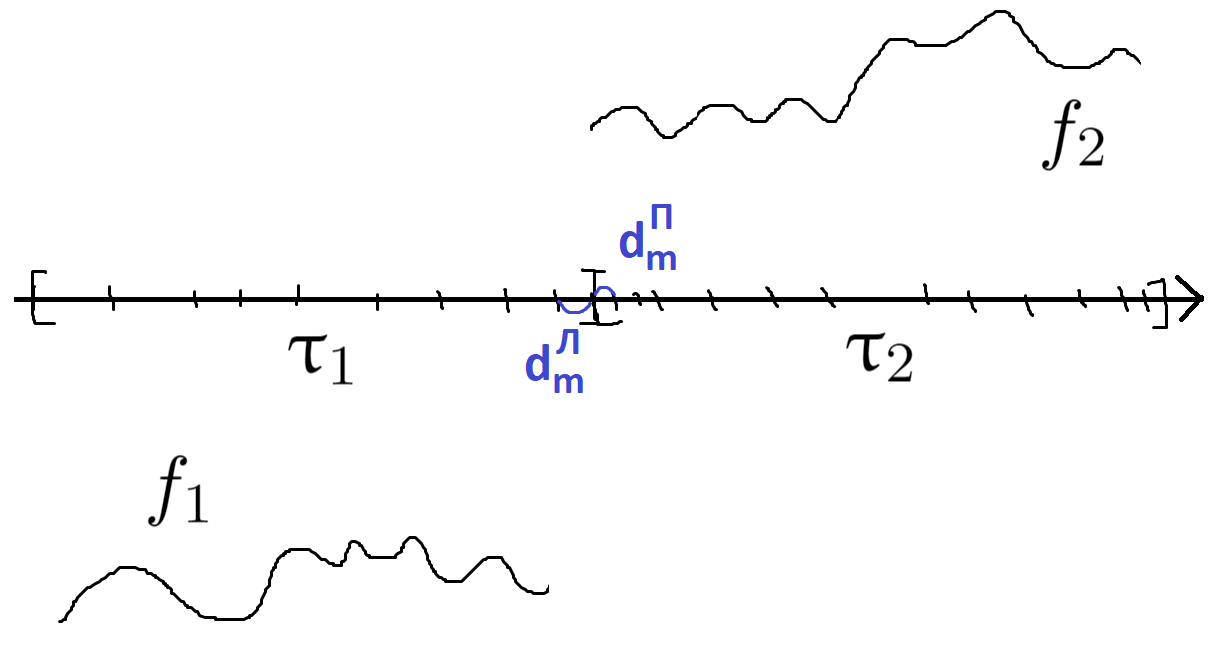
\includegraphics[scale=0.3]{8_1}

      Мог произойти разрыв, но $|f| \leqslant M \Rightarrow \upomega(f,[a,b]) \leq W$
      $$\sum \upomega(f,d_k)\Delta_k = S^*(f, \uptau)-S_*(f, \uptau) \leqslant S^*(f, \uptau_1)-S_*(f, \uptau_1) + S^*(f, \uptau_2)-S_*(f, \uptau_2) + $$
      $$+d_m^\text{Л} \Delta_m^\text{Л} + d_m^\text{П} \Delta_m^\text{П} \leqslant (d_m=d_m^\text{Л} \cup d_m^\text{П},\ \w{\updelta}=\min(\updelta_1, \updelta_2, \frac{\E}{W})) 2 \E + W \w{\updelta} < 3 \E$$
  \end{proof}

  \newpage
  \section{Свойства интеграла Римана (линейность; аддитивность; свойства, связанные с неравенствами).}

  \begin{definition}
      Если $a < b$, то  $\int\limits^a_b f=-\int\limits^b_a f$ и $\int\limits^a_a = 0$
  \end{definition}

  \begin{Property}[1, линейность]
      \[\forall f,g \in R[a,b], \upalpha, \upbeta \in \R \Rightarrow \int\limits^a_b (\upalpha f + \upbeta g) = \upalpha \int\limits^a_b f + \upbeta \int\limits^a_b g\]
  \end{Property}

  \begin{proof}
      Знаем, что $\upalpha f + \upbeta g \in R[a,b],$
      $$S(\upalpha f + \upbeta g,  \uptau, \xi) = \upalpha S(f, \uptau, \xi) + \upbeta S(g,  \uptau, \xi) \text{ (очевидно из определения сумм Римана)}$$
  \end{proof}

  \begin{Property}[2, аддитивность]
      \[\forall f \in R[a,b],\ a<c<b \Rightarrow \int\limits^a_b f = \int\limits^a_c f + \int\limits^c_b f\]
  \end{Property}

  \begin{proof}
  Очевидно (аналогично прошлому)
  \end{proof}

  \begin{Property}[3]
      \[\forall f \in R[a,b],\ a<b,\ f \geqslant 0 \Rightarrow \int\limits_a^b f \geqslant 0\]
  \end{Property}

  \begin{proof}
      Очевидно из определения суммы Римана
  \end{proof}

  \begin{Property}[4]
      \[\forall f,g \in R[a,b],\ g(x) \leqslant f(x)\ \forall x \in [a,b], a<b \Rightarrow \int\limits^a_b g \leqslant \int\limits^a_b f\]
  \end{Property}

  \begin{proof}
      Очевидно, если взять одно разбиение и оснащение
  \end{proof}

  \begin{Property}[5]
      \[\forall f \in R[a,b],\ m \leqslant f(x) \leqslant M\ \forall x \in [a,b], a<b \Rightarrow m(b-a) \leqslant \int\limits^a_b f \leqslant M(b-a)\]
  \end{Property}

  \begin{proof}
      С использованием предыдущего свойства взять интеграл
  \end{proof}

  \begin{Property}[6]
      \[f \in R[a,b],\ m = \inf\limits_{[a,b]} f,\ M = \sup\limits_{[a,b]} f \Rightarrow \e \upmu \in [m,M]: \int\limits^a_b f =\upmu (b-a)\]
  \end{Property}

  \begin{Proof}
      \[\upmu=\frac{\int\limits^a_b f}{b-a} \in [m,M] \text{ (по предыдущему неравенству)}\]
  \end{Proof}

  \begin{Property}[7]
      \[f \in C[a,b], \Rightarrow \e \xi \in [a,b]: \int\limits^a_b f = f(\xi) (b-a)\]
  \end{Property}

  \begin{proof}
      По теореме о промежуточном значении (Больцано-Коши) используя предыдущее свойство
  \end{proof}

  \begin{Property}[8]
      \[f \in R[a,b], \Rightarrow |\int\limits^a_b f| \leqslant \int\limits^a_b |f|\]
  \end{Property}

  \begin{proof}
      $-|f| \leqslant f \leqslant |f| \Rightarrow -\int\limits^a_b |f| \leqslant \int\limits^a_b f \leqslant \int\limits^a_b |f| \Rightarrow |\int\limits^a_b f| \leqslant \int\limits^a_b |f|$
  \end{proof}

  \newpage
  \section{Первая теорема о среднем. Следствие для непрерывных функций.}

  \begin{Theorem}
      \[f,g \in R[a,b],\ g \geqslant 0,\ m \leqslant f \leqslant M\] \[\forall x \in [a,b] \Rightarrow \e \upmu \in [m,M]: \int\limits^a_b f g = \upmu \int\limits^a_b g\]
  \end{Theorem}

  \begin{proof}
      $m g \leqslant f g \leqslant Mg \Rightarrow m \int\limits^a_b g \leqslant \int\limits^a_b f g \leqslant M \int\limits^a_b g$
      \[\frac{m \int_b^a g}{\int_b^a g} \leq \frac{\int_b^a fg}{ \int_b^a g} \leq \frac{M \int_b^a g}{\int_b^a g}\]
    \[m \leq \frac{\int_b^a fg}{\int_b^a g} \leq M\]
      а) $\int\limits^a_b g = 0$, тогда $\upmu$ - любое.\\
      б) $\int\limits^a_b g \neq 0 \Rightarrow \upmu:=\frac{\int\limits^a_b f g}{\int\limits^a_b g} \in [m,M]$
  \end{proof}

  \begin{consequence}
      Eсли $f \in C[a,b],\ g \in R[a,b],\ g \geqslant 0 \Rightarrow \e \xi \in [a,b]: \int\limits^a_b f g = f(\xi) \int\limits^a_b g$
  \end{consequence}


  \begin{proof}
      По теореме о промежуточном значении (Больцано-Коши) используя неравенство из последнего доказательства для $m=\inf\limits_{[a,b]} f,\ M=\sup\limits_{[a,b]} f$
  \end{proof}
\end{document}
